The assignment solution consists of a video game, two linux character drivers, as well as a suite of various tools and scripts.
The solution video game is a rhythm video game and is controlled using the STK1000's buttons.
The LEDs are used to indicate which buttons are relevant at the different stages of the game.

\subsection{The gameplay of Scorched Land Dance Dance Defence}
	\subsubsection{The role of the LEDs}
		The LEDs are used to indicate which buttons that can be pressed in each state.
		For example: during gameplay \texttt{LED7}, \texttt{LED5}, \texttt{LED3} and \texttt{LED2} are lit, corresponding to the buttons used to play the game.
	\subsubsection{Splash screen}
		The \textit{splash screen} is the first screen displayed to the player.
		It states the name of the game and displays a nice-looking real-time flame effect, tying in nicely with the name of the game.
		Pressing \texttt{SW3} advances the game to the \textit{song selection menu}.
		An image of the splash screen can be seen in figure \ref{img-splashscreen}.
		\begin{figure}[h]
			\centering
			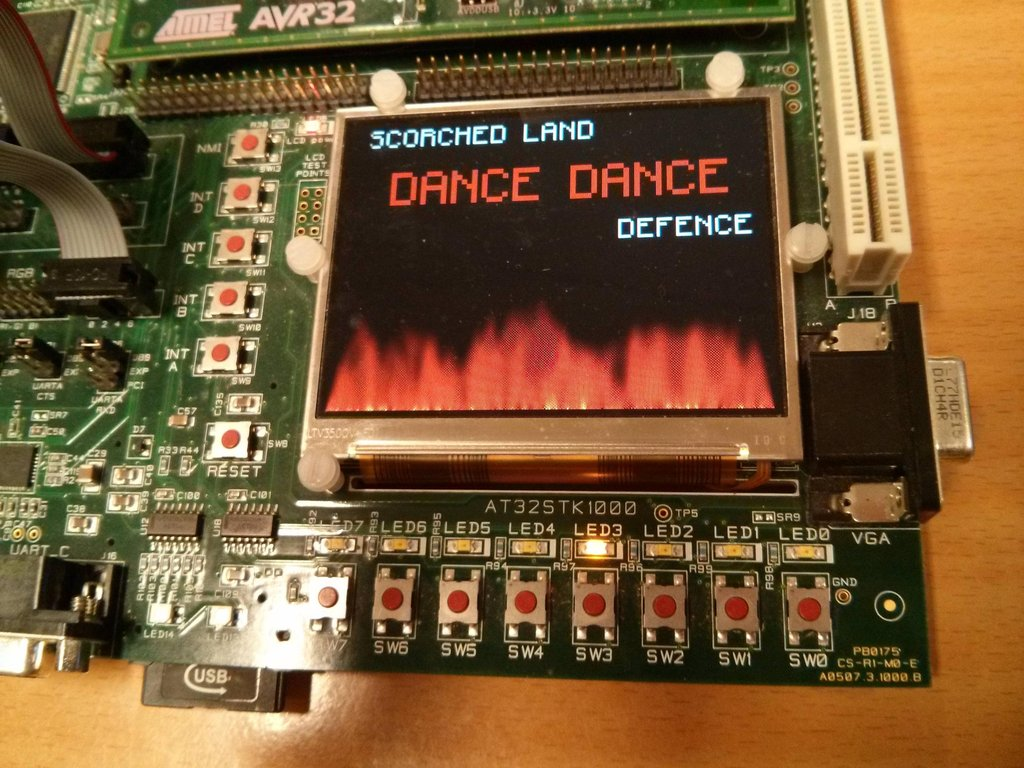
\includegraphics[width=4in]{{images/gameplay-splashscreen.jpg}}
			\caption{SLDD's splash screen.}
			\label{img-splashscreen}
		\end{figure}
	\subsubsection{Song selection menu}
		This is the menu from which the player selects which song he or she wishes to play.
		Pressing \texttt{SW3} selects the highlighted song, while pressing \texttt{SW2} traverses the list one song upwards and \texttt{SW1} traverses the list one song downards.

		In addition to \texttt{LED1}, \texttt{LED2} and \texttt{LED3} being lit when this screen is active, three icons are visible in the bottom right hand corner of the screen.
		These indicate the consequence of pushing the corresponding buttons.
		An image of the song selection menu can be seen in figure \ref{img-songselect}.
		\begin{figure}[h]
			\centering
			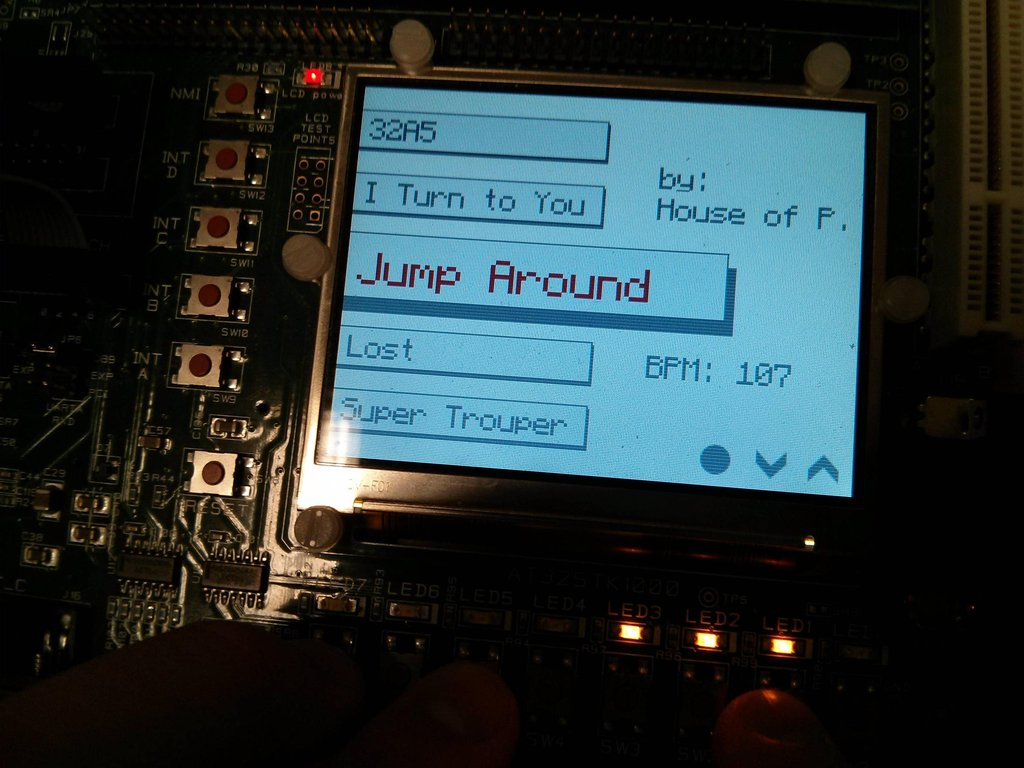
\includegraphics[width=4in]{{images/gameplay-songselect.jpg}}
			\caption{The song selection menu of SLDDD. In this image, "Jump Around" by House of P. is hightlighted.}
			\label{img-songselect}
		\end{figure}
	\subsubsection{In-song gameplay}
		When a song is selected in the \textit{song selection menu}, the game begins the in-song gameplay mode. This mode is pictured in figure~\ref{img-insong}.
        In this mode, the selected song plays on the speakers whilst red hexagon fly across the screen in a rythmical manner. 
		The song's background image is rendered with a slightly transparent overlay of four white rectangles each with a hexagon outlined at the top.
        The objective of the game is to press the appropriate buttons in the rhythm defined by the moving red hexagon as they pass over the grey hexagon outlines.

		\texttt{SW7} corresponds to the leftmost stationary hexagon, \texttt{SW5} to the second one from the left, \texttt{SW3} to the second one from the right and \texttt{SW1} to the rightmost.
		A judgment is given for each moving hexagon, depending on how close it is to its corresponding stationary hexagon when the appropriate button is pressed.
		The given judgments are displayed at the top of the screen as the game progresses, and a combo counter hovers above the game area when a player is in the middle of a combo.
        \footnote{A combo is defined as a number of successive successful rhythmical taps of the buttons.}
		
		Judgments are calculated from the moving hexagon's pixel offset from the stationary hexagon, see table~\ref{table-judgments} for a full list.
		\begin{table}[h]
			\centering
		    \begin{tabular}{|l|l|}
		    \hline
		    Judgment & Timing (offset in pixels) \\ \hline
		    PERFECT! & [0,3] \\ \hline
		    Great! & [4,9] \\ \hline
		    O.K. & [10,19] \\ \hline
		    \end{tabular}
		    \caption{The judgments in SLDDD and their offsets.}
		    \label{table-judgments}
		\end{table}
	
		When the song is finished the game advances to the \textit{score screen}.
		Pressing \texttt{SW0} causes the game to return to the \textit{song selection screen}.
		\begin{figure}[h!]
			\centering
			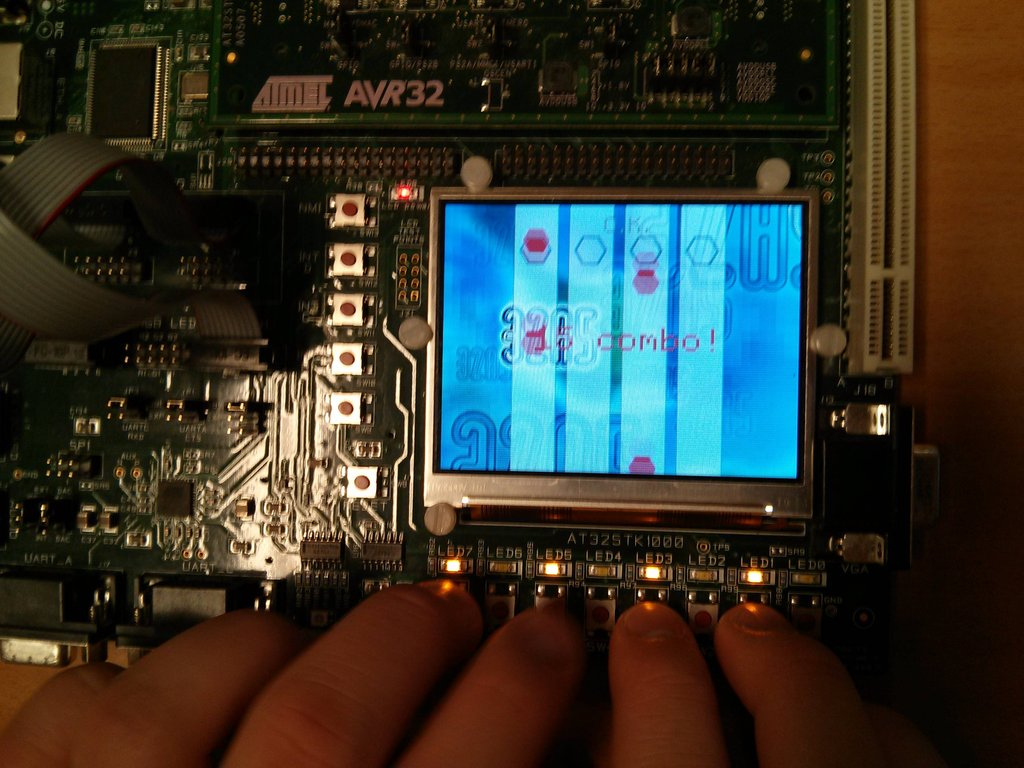
\includegraphics[width=4in]{{images/gameplay-insong.jpg}}
			\caption{The in-song interface of SLDD. The song being played here is ``Jump Around''.}
			\label{img-insong}
		\end{figure}
	\subsubsection{Score screen}
		The \textit{score screen} summarizes the player's performance in a song.
		An enumeration of each judgment, the player's highest combo count during the song as well as an overall score are displayed here.
		The score is calculating by adding the number of perfects, greats and O.K.s multiplied with their weights. Perfect is weighted 8, great has a weight of 5 and O.K. has a weight of 3.

		Pressing \texttt{SW0} returns to the \textit{song selection screen}.
		\begin{figure}[h!]
			\centering
			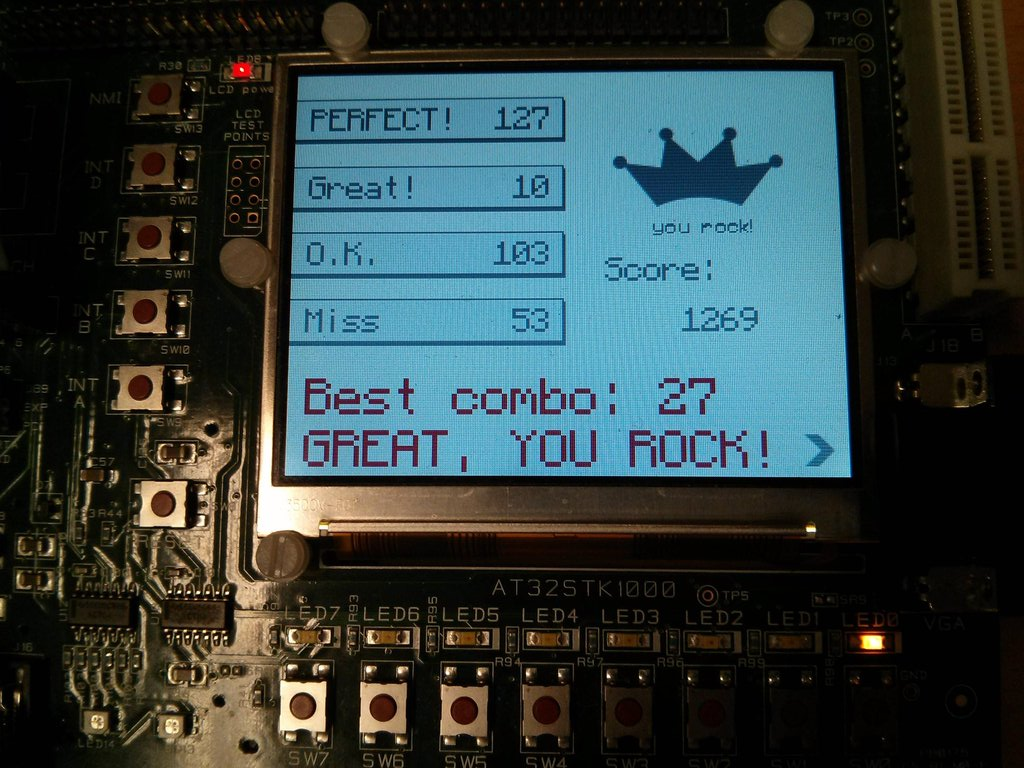
\includegraphics[width=4in]{{images/gameplay-scorescreen.jpg}}
			\caption{SLDDD's score screen. The song played was ``Jump Around''.}
			\label{img-scorescreen}
		\end{figure}
